\documentclass{article}
\usepackage{pdfpages}   % 插入PDF必备
\usepackage{ctex}       % 支持中文（必须加！）
\usepackage{fontspec}
\usepackage{tocloft}    % 目录定制工具包
\usepackage{fancyhdr}   % 页眉页脚宏包
% 页面大小、边距（可选，让排版更舒服）
\usepackage{geometry}
\usepackage{graphicx}   % 插入校徽图片
\usepackage{setspace}   % 调整行间距
\usepackage{longtable}
\usepackage{caption}
\usepackage{graphicx}  % 图片支持
\usepackage{float}     % 如需 H 位置
\usepackage{amsmath}

\captionsetup{labelsep=space}  % 将冒号改为空格

\geometry{a4paper, margin=2.5cm} % 调整页边距，让封面居中更好看

% ========== 核心：只修改 section 编号为“第X章”，其他层级不变 ==========
\renewcommand{\thesection}{第\chinese{section}章}
\renewcommand{\thesubsection}{\arabic{section}.\arabic{subsection}}
\renewcommand{\thesubsubsection}{\arabic{section}.\arabic{subsection}.\arabic{subsubsection}}

% ========== 目录标题格式：黑体、二号、居中，下空一行 ==========
\renewcommand{\contentsname}{\centering\heiti\zihao{2} 目录}
\renewcommand{\cfttoctitlefont}{\centering\heiti\zihao{2}}
\renewcommand{\cftaftertoctitle}{\vspace{1em}}

% ========== 目录内容格式：小四号、行距20磅 ==========
\renewcommand{\cftsecfont}{\bfseries\heiti\zihao{-4}}    % section（第一章）黑体加粗
\renewcommand{\cftsecpagefont}{\bfseries\heiti\zihao{-4}}
\renewcommand{\cftsubsecfont}{\songti\zihao{-4}}         % subsection 宋体
\renewcommand{\cftsubsecpagefont}{\songti\zihao{-4}}
\renewcommand{\cftsubsubsecfont}{\songti\zihao{-4}}      % subsubsection 宋体
\renewcommand{\cftsubsubsecpagefont}{\songti\zihao{-4}}

% ========== 解决文字重叠问题：给“第X章”预留足够宽度 ==========
\setlength{\cftsecnumwidth}{4.5em}   % 给“第1章”预留宽度，避免和标题重叠
\setlength{\cftsubsecnumwidth}{2.5em} % 给“1.1”预留宽度
\setlength{\cftsubsubsecnumwidth}{3.5em} % 给“1.1.1”预留宽度

% ========== 调整目录编号与标题之间的间距 ==========
\renewcommand{\cftsecpresnum}{}
\renewcommand{\cftsecaftersnum}{\quad}  % “第1章”和标题之间加一个空格
\renewcommand{\cftsubsecpresnum}{}
\renewcommand{\cftsubsecaftersnum}{\quad}
\renewcommand{\cftsubsubsecpresnum}{}
\renewcommand{\cftsubsubsecaftersnum}{\quad}

% ========== 显示到三级目录 ==========
\setcounter{tocdepth}{3}

% ========== 正文 section 标题格式：小二号黑体、居中 ==========
\usepackage{titlesec}
\titleformat{\section}
{\centering\heiti\zihao{2}} % 居中 + 黑体 + 小二号
{\thesection}               % 显示 第一章
{1em}                        % 编号与标题间距
{}

\titleformat{\subsection}
{\normalfont\raggedright\heiti\zihao{4}}  % 强制左对齐，黑体，四号
{\thesubsection}
{1em}
{}

\titleformat{\subsubsection}
{\normalfont\raggedright\heiti\zihao{-4}} % 强制左对齐，黑体，小四
{\thesubsubsection}
{1em}
{}

\titlespacing*{\section}{0pt}{2em}{1em}
\titlespacing*{\subsection}{0pt}{1.5em}{0.5em}
\titlespacing*{\subsubsection}{0pt}{1em}{0.3em}

% 加下面这一句 ！！！
\let\bfseries\mdseries

% ========== 清除 fancyhdr 原有的章节标记，避免冲突 ==========
% （article 类的 section 标记默认只写编号，需要重定义）
\renewcommand{\sectionmark}[1]{%
	\markboth{\thesection \ #1}{}%
}

% ========== 自定义「正文页」样式 ==========
\fancypagestyle{mainstyle}{
	\fancyhf{}                                    % 清空所有页眉页脚
	\fancyhead[L]{面向多模态理解任务的ViT自适应Token裁剪}       % 左页眉：论文标题
	\fancyhead[R]{\leftmark}                      % 右页眉：第X章 章节标题
	\fancyfoot[C]{\thepage}                       % 页脚居中：页码
	\renewcommand{\headrulewidth}{0.5pt}           % 页眉线 0.5pt
}

% ========== 章节首页样式（默认无页眉，但页脚保留页码） ==========
\fancypagestyle{plain}{                           % 重定义 plain 样式
	\fancyhf{}
	\fancyfoot[C]{\thepage}
	\renewcommand{\headrulewidth}{0pt}             % 章节首页不要页眉线
}



\begin{document}
	
	% ========================
	% 1. 第一页：封面（这里由于需要填信息所以手动制作封面，不直接导入pdf）
	% ========================
	\thispagestyle{empty} % 封面不显示页码
	\centering % 整体居中
	% 校名（书法字体）
	
\includegraphics[height=3.22cm]{name.png} % 控制校名图片高度，适配模板大小
	
	% 论文类型（本科毕业论文（设计））
	\fontsize{35}{42}\selectfont \heiti 本科毕业论文（设计）\\
	\vspace{0.2cm}
	% 校徽（需要你把校徽图片命名为 fdu-logo.png 和 tex 文件放一起）
	
\includegraphics[width=3.68cm]{fdu-logo.png} % 替换成你的校徽文件路径
	\vspace{1.0cm}
	
	% 论文题目：整体小三黑体；题目内容小二黑体加粗
	\begin{flushleft}
		{\heiti\zihao{-3} 论文题目：%
			\quad {\heiti\zihao{-2}\bfseries 面向多模态理解任务的ViT自适应Token裁剪}}
	\end{flushleft}
	
	% 个人信息：全部小三黑体；两列布局
	\begin{flushleft}
		{\heiti\zihao{-3}
			\begin{tabular}{@{}l@{\hspace{8em}}l@{}}
				\makebox[5em][s]{姓名：}\quad 戚子祥             & \makebox[5em][s]{学号：}\quad 19301020017 \\[1.2em]
				\makebox[5em][s]{院系：}\quad 计算与智能创新学院 & \\[1.2em]
				\makebox[5em][s]{专业：}\quad 计算机科学与技术   & \\[1.2em]
				\makebox[5em][s]{指导教师：}\quad 陈智能         & \makebox[5em][s]{职称：}\quad 教授 \\[1.2em]
				\makebox[5em][s]{单位：}\quad 复旦大学           & \\[1.2em]
				\makebox[5em][s]{完成日期：}\quad 2026 年 5 月 12 日 & 
			\end{tabular}}
	\end{flushleft}
	
	\clearpage % 封面结束，进入下一页正文
	
	% ========================
	% 2. 中间：你的所有内容（目录、摘要、正文）
	% ========================
	% 从这里开始，就是你自己的论文内容
	\pagenumbering{Roman}         % 罗马数字页码：I, II, III...
	\setcounter{page}{1}          % 从 I 开始
	\pagestyle{plain}             % 目录页无页眉，仅页脚居中页码
	
	{
		\parskip=0pt
		\fontsize{12}{20}\selectfont % 这里 12 只是一个占位字号；真正字号仍会被你 cftsecfont 等覆盖
		\tableofcontents
	}%固定目录的行距为正常值20磅
	\newpage                % 分页
	
	\thispagestyle{empty} % 摘要不显示页码
	\centering          % 居中
	\fontsize{18}{22}\heiti 摘要  % 小二号黑体、居中
	\par
	\vspace{1em}        % 标题下方空一行
	
	% 摘要内容：小四号宋体，行距20磅，首行缩进2字符
	\begingroup
	\raggedright
	\fontsize{12}{20}\selectfont  % 小四号（12pt），行距固定20磅
	\setlength{\baselineskip}{20pt} %行距设置为20磅
	\setlength{\parindent}{2em}   % 首行缩进2个字
	\songti  % 宋体
	近年来，视觉Transformer在图文检索、视觉问答、图文推理等多模态理解任务中表现出了较强的能力，但是由于计算开销比较大，限制了其在资源受限场景中的应用。针对上述问题，本文围绕视觉token的自适应裁剪展开研究，目的是探索一种无需额外标注并且无需专门训练的token重要性估计方法，并进一步研究可训练的gating head在多任务场景下的适配效果。本文以OpenCLIP中的视觉编码器Vit-B/32为基础，在图文检索、视觉问答、图文推理三个任务上展开实验，使用的数据集分别是Flickr30k、ScienceQA、Winoground。实验中，采用基于CLS token与所有patch token注意力分数的启发式裁剪策略，并与L2范数打分的方法进行比较。同时在此基础上也进一步构建了gating head，对视觉token进行可学习评分，并结合了软裁剪预训练 + 模型微调 + 硬裁剪推理，验证了其对不同任务性能与效率的影响。实验结果表明，使用CLS-attention进行裁剪能够在保持任务性能的同时有效减少token数量，以达到降低计算量的目的。经过gating head训练和微调后，模型在部分任务上可获得更优的性能-效率折中。本文的研究表明，视觉token的重要性可以借助模型内部注意力信息进行有效估计，且该策略在多种多模态理解任务中具有一定迁移性和实用价值。
	\par
	\endgroup
	\vspace{1em}        % 空一行
	
	% 关键词：小三号黑体 + 小四号宋体
	\raggedright
	\noindent\fontsize{15}{18}\heiti 关键词：
	\fontsize{12}{15}\selectfont\songti 视觉Transformer,\fontsize{12}{15}\selectfont 图文检索,\fontsize{12}{15}\selectfont\songti 视觉问答,\fontsize{12}{15}\selectfont 图文推理,\fontsize{12}{15}\selectfont\songti token裁剪
	% 关键词5个，逗号分隔，最后无标点
	
	% ---------------------
	% 英文摘要（与中文对应）
	% ---------------------
	\newpage
	\thispagestyle{empty} % 摘要不显示页码
	\centering
	\fontsize{18}{22}\bfseries ABSTRACT  % 英文题目全大写，小二号、居中
	\par
	\vspace{1em}
	
	\begingroup
	\raggedright
	\fontsize{12}{20}\selectfont
	\setlength{\baselineskip}{20pt}
	\setlength{\parindent}{0pt} %英文摘要不用首行缩进
	In recent years, Vision Transformers have demonstrated strong capabilities in multimodal understanding tasks such as image-text retrieval, visual question answering, and image-text reasoning. However, their high computational cost limits their application in resource-constrained scenarios. To address this problem, this thesis investigates adaptive pruning of visual tokens, aiming to explore a token importance estimation method that requires neither additional annotations nor task-specific training, and to further study the adaptability of a trainable gating head in multi-task settings. Based on the ViT-B/32 visual encoder in OpenCLIP, experiments are conducted on three tasks: image-text retrieval, visual question answering, and image-text reasoning, using the Flickr30k, ScienceQA, and Winoground datasets, respectively. In the experiments, a heuristic pruning strategy based on the attention scores between the CLS token and all patch tokens is adopted and compared with an L2-norm-based scoring method. On this basis, a gating head is further constructed to assign learnable scores to visual tokens, and a training scheme combining soft pruning pretraining, model fine-tuning, and hard pruning inference is introduced to evaluate its impact on task performance and efficiency. Experimental results show that CLS-attention-based pruning can effectively reduce the number of tokens while maintaining task performance, thereby lowering computational cost. After training and fine-tuning the gating head, the model achieves a better performance-efficiency trade-off on some tasks. The results indicate that the importance of visual tokens can be effectively estimated by the model’s internal attention signals, and that the proposed strategy has certain transferability and practical value across multiple multimodal understanding tasks.
	\par
	\endgroup
	\vspace{1em}
	
	\raggedright
	\begingroup
	% 1. 标题：小三号（14pt）加粗，对应中文的“小三号黑体”
	\fontsize{16}{19}\bfseries KEY WORDS:
	% 2. 关键词：小四号（12pt）正常字体，和中文关键词字号一致
	\fontsize{12}{15}\selectfont VISION TRANSFOMER, IMAGE-TEXT RETRIEVAL, VISUAL QUESTION ANSWERING, IMAGE-TEXT REASONING, TOKEN PRUNING
	\endgroup
	
	\newpage
	% 正文开始
	%                     正 文 部 分（从引言开始）
	% ================================================================
	\pagenumbering{arabic}        % 切换为阿拉伯数字页码
	\setcounter{page}{1}          % 重新从 1 开始
	\pagestyle{mainstyle}         % 启用正文页眉页脚样式
	
	
	\section{引言}
		\subsection{课题背景与研究意义}
		{\zihao{-4}\setlength{\parindent}{2em}\setlength{\baselineskip}{20pt}\selectfont
			随着多模态人工智能的发展，图像与文本联合建模已经成为视觉理解领域的重要研究方向。基于Transformer架构的视觉模型，尤其是ViT及其在CLIP中的应用，能够通过全局建模捕获图像中的丰富语义信息，在图文检索、视觉问答、图文推理等任务中均取得了较好的效果。然而，ViT在处理图像时需要对大量patch token进行逐层计算，这会带来比较高的计算复杂度，尤其是在多任务联合评测或者部署到实际系统的情况下，这一问题便会更加突出。因此，如何在尽量不损害模型性能的前提下剔除冗余token，降低计算开销，就成了多模态模型高效推理的重要研究问题。
		\subsection{研究目的}
		{\zihao{-4}\setlength{\parindent}{2em}\setlength{\baselineskip}{20pt}\selectfont
			本文旨在研究一种适用于多种多模态理解任务的ViT自适应token裁剪方法。具体目标包括：在不依赖额外监督标注的条件下，利用模型内部信息评估视觉token的重要性；分析不同多模态任务对token保留程度的敏感性；在此基础上进一步探索可学习的gating head是否能够相较于启发式裁剪获得更优的性能与效率平衡。通过在图文检索、视觉问答和图文推理三类任务上的系统实验，验证文中提出方法的有效性与泛化能力。
		\subsection{研究内容与核心方法}
		{\zihao{-4}\setlength{\baselineskip}{20pt}\selectfont
			\setlength{\parindent}{2em}本文以OpenCLIP中的视觉编码器ViT-B/32为基础，围绕视觉token裁剪展开研究，主要包括以下几个方面：\setlength{\parindent}{0em}
			\\
			1)以Flickr30k图文检索任务为基础，分析不同层进行token裁剪时对召回性能的影响，并比较L2范数打分与CLS attention打分两类策略；\\
			2)在ScienceQA视觉问答任务上，验证CLS attention裁剪策略在分类准确率与推理速度上的表现，并寻找任务对应的较优裁剪配置；\\
			3)在Winoground图文推理任务上，研究token裁剪对细粒度视觉推理能力的影响，分析剪枝层和保留比例对性能与速度的权衡；\\
			4)在启发式裁剪的基础上，进一步设计轻量级gating head，通过软裁剪训练+微调+硬裁剪推理，学习token评分并提升跨任务适配能力。
		\subsection{论文结构}
		{\zihao{-4}\setlength{\parindent}{2em}\setlength{\baselineskip}{20pt}\selectfont
			本文的组织结构如下：
			第一章为引言，介绍研究背景、意义、主要内容和论文结构；
			第二章对国外文献资料进行分析和综述；
			第三章介绍相关理论基础与前导知识，包括ViT、CLIP及token裁剪相关方法；
			第四章分析系统需求并给出总体设计；
			第五章详细介绍启发式CLS-attention裁剪方法及实验设置，同时介绍gating head的设计、训练与微调方法；
			第六章对图文检索、视觉问答和图文推理三个任务的实验结果进行分析与总结；
			第七章总结全文并展望未来工作。
	\section{国外文献资料的分析和综述}
	{\zihao{-4}\setlength{\parindent}{2em}\setlength{\baselineskip}{20pt}\selectfont
		近年来，Transformer架构在计算机视觉各类研究场景中已深度普及，视觉Transformer（ViT）逐渐成为图像特征学习领域的一类核心基础模型。不同于卷积神经网络只能局限于局部区域提取特征，ViT采取了分块编码的策略：把完整图像拆成多个序列化的补丁单元，再利用自注意力机制来捕捉全局范围的依赖关系。整体上，其适配能力更强，目前已在图像分类、目标检测、图像检索以及多模态语义理解等主流视觉任务中得到广泛应用。\\
		在多模态建模研究里，CLIP、OpenCLIP这类经典视觉语言预训练模型，也都把ViT用作视觉端编码器，再配合文本编码器一起做跨模态联合表征学习。图文检索、视觉问答、图文推理等下游任务的能力因此稳步提升。不过，ViT有一个现实问题：它的全局密集交互结构导致算力开销偏大、推理速度偏慢。针对这一点，国内外学界把攻关重点放在了冗余Token的优化提速上。现有的主流提速方案大致分为三类，分别是基于重要性评分筛选、基于注意力权重分布调控，以及基于可学习门控的自适应裁剪。\\
		在基于重要性评分的优化路径上，早期研究大多依靠Token特征的范数值、激活响应强度或者梯度变化信息，直接判断各个图像补丁的重要程度，然后把贡献较低的Token剔除掉。这类方法结构比较简单，部署起来也方便，不需要额外的标注数据来做辅助训练，通用性整体上不错。但问题在于，评判指标的维度比较单一，贴合度也不太够，没法精准适配不同任务场景里Token对模型决策的真实影响。已有的研究已经证明，如果只靠特征幅值去做硬性裁剪，很容易忽略Token之间那种紧密的上下文关联。尤其是在细粒度视觉识别任务里，一旦过度删减有效Token，关键细节信息就可能丢失，模型综合识别性能会明显下降。\\
		另一类主流方案，是利用Transformer原生自带的注意力分布来评估Token优先级。自注意力机制本身就能比较直观地反映不同补丁之间的信息交互强度，所以学界普遍的做法是，结合全局CLS Token和各个图像Patch Token之间的关联注意力权重，设计裁剪策略。不少实验发现，CLS Token在全程聚合全图的全局语义，那些与CLS注意力关联度越高的Patch，通常承载着图像里的核心目标和关键场景信息。基于这一规律，研究人员一般会保留高注意力权重的Token，剔除低权重的冗余单元，从而降低模型计算压力。相比于传统那种基于范数的剪枝方法，这个做法更贴合模型内部语义流动的逻辑，不需要额外训练调优，就能在表征精度和推理效率之间做一个比较好的平衡，综合优势比较明显。\\
		另外，也有不少研究把Token裁剪策略和可学习门控机制结合到一起，用一个轻量化的专属评分网络来自适应地判定每个输入、每个任务下的Token留存优先级。相比那些固定的人工启发式规则，这种做法能更灵活地适配不同的下游任务和复杂的样本场景，裁剪时的贴合度更高。常见实现方式包括，逐Token拟合动态重要性分数，或者在Transformer编码层内部插入门控筛选模块，精准过滤掉无效的中间表征。这种方法的建模比较灵活，多任务适配性也强，适合用在复杂的高阶视觉推理场景里。但它也有明显短板：新增训练模块会占掉一部分算力成本，还会增加结构设计难度，推理阶段也容易出现表征不稳定。对大规模视觉预训练模型来说，在尽量不破坏原有核心能力的前提下，低成本地嵌入可学习裁剪模块，目前仍然是一个不太好解决的技术难点。\\
		放到多模态理解的专属场景来看，相关研究主要是在优化视觉和文本双编码器协同建模过程中的整体推理效率。CLIP这类跨模态预训练模型虽然图文对齐能力不错，但视觉分支依然存在编码Token数量偏多、算力资源浪费较严重的问题。针对这个问题，学界开始尝试动态Token裁剪策略，把它用到图文检索、视觉问答、图文推理这些多模态核心任务里，减少视觉编码环节里那些冗余无效的计算。实际测试数据表明，不同的多模态任务对Token裁剪比例的耐受程度差别挺大。检索类的任务容错性更强一些，而视觉推理类的任务对局部细节的完整性要求更高。这就意味着，轻量化裁剪设计不能只顾着提速降耗，还得紧密贴合具体任务的语义表征需求，做到定制化的适配。\\
		整体上看，现阶段ViT Token裁剪相关的研究已经形成了一条比较清晰、相对完整的技术路线。一条路是依托模型原生自带的各种隐式或显式特征信号，做启发式的静态裁剪。另一条路是借助可学习门控网络，做动态自适应的Token筛选。还有一条路是面向不同的应用场景，在精度和推理效率之间做平衡，定制化设计轻量化方案。现有方法在图像分类这类基础视觉任务上已经落地得比较成熟，但针对多模态复杂理解任务的系统性专项研究，还是偏少。到现在为止，CLS注意力能不能作为一个通用的Token评判指标，还没有被充分验证。可学习门控机制在多个多模态下游任务里的迁移适配能力，也缺少实际测试的支撑。因此，面向多模态理解场景去研发ViT自适应Token裁剪方法，既能解决大模型落地时算力受限的工程难题，也能丰富多模态轻量化方面的研究体系，具备较高的应用价值和学术意义。
	\section{前导知识简介}
	{\zihao{-4}\setlength{\parindent}{2em}\setlength{\baselineskip}{20pt}\selectfont
		本章面向多模态理解场景下的视觉Token裁剪技术，进行基础理论方面的铺垫。内容主要涉及几个方向：视觉Transformer架构、视觉语言预训练模型、注意力机制原理、Token重要性评估方式，以及模型轻量化加速技术。为了便于后续算法设计和实验分析，本节对这些关键技术逐一做了梳理和说明。
		\subsection{视觉Transformer}
		{\zihao{-4}\setlength{\parindent}{2em}\setlength{\baselineskip}{20pt}\selectfont
			Transformer架构最早是用在自然语言处理领域的。它的核心是靠自注意力机制来建模序列元素之间的远距离关联，这一点正好补上了传统循环结构在长距离依赖建模上的短板。后来有研究者把这个架构往计算机视觉领域迁移，视觉Transformer（ViT）模型就这么出来了。ViT的基本思路不算复杂：把一张完整的图像均匀切成多个大小一样的图像小块，每个小块被映射成一个独立的特征Token，然后把这些Token以序列的形式送进Transformer编码器，做全局特征建模。传统卷积神经网络得靠局部卷积核一层一层提特征，ViT不一样，它不受局部感受野的限制，可以直接建立整个图像范围内的长距离关联。从提取全局语义特征这个角度看，ViT有天然的优势。\\
			再看ViT的整体结构。里面额外嵌入了一个CLS Token，专门负责汇总整张图的全局语义特征。剩下的那些Patch Token，各自对应图像里局部区域的细节特征。随着网络编码层数不断加深，CLS Token会不停地融合各个Patch Token的关键信息，慢慢生成更高阶的全局语义表征。这就意味着，CLS Token和各个Patch Token之间的注意力权重分布，能比较直观地反映出不同图像区域对当前视觉任务有多大贡献。这个观察为本研究提供了底层理论支撑——我们后面就是依托CLS注意力信号来设计Token裁剪方案的。
		\subsection{视觉-语言预训练模型}
		{\zihao{-4}\setlength{\parindent}{2em}\setlength{\baselineskip}{20pt}\selectfont
			视觉语言预训练模型的核心做法是，拿大规模的图文成对数据做跨模态联合训练。目标也很明确：建立图像和文本之间精准的语义对齐关系，让模型具备比较强的跨模态迁移泛化能力。CLIP是这个方向上一个很有代表性的经典模型。它的架构由独立的视觉编码器和文本编码器并行组成，各自负责提取图像视觉特征和文本语义特征。训练的时候用的是对比学习范式——匹配的图文对，特征空间距离不断拉近；不匹配的图文样本，特征距离被拉大。通过这种方式，跨模态匹配能力逐步增强。OpenCLIP是在CLIP原生架构基础上优化迭代出来的一个开源衍生版本，训练流程和部署适配逻辑都做了改进，用起来更灵活。\\
			相比那些只能处理单一场景的传统视觉模型，CLIP系列模型既能做高精度的图像特征提取，又能理解自然语言语义。像图文跨模态检索、实景视觉问答、细粒度图文推理这类下游任务，它都能直接适配，通用性比较强。本文选择OpenCLIP框架下的ViT-B/32作为核心实验基线模型。原因有两个：一是它的表征建模能力比较均衡，二是在行业里有比较好的通用代表性，用来评估不同视觉Token裁剪策略在多模态复杂场景下的适配性能，结果会比较客观。
		\subsection{注意力机制与CLS Token}
		{\zihao{-4}\setlength{\parindent}{2em}\setlength{\baselineskip}{20pt}\selectfont
			注意力机制是Transformer架构里一个核心的驱动模块。它的运行逻辑大致是这样：根据输入序列里不同单元的关联紧密程度，动态分配权重资源，引导模型先关注那些高价值的关键信息区域。自注意力机制算是其中一个主要分支，它能对序列中所有Token做两两之间的双向关联建模，捕捉全局范围的长距离依赖关系，从而提升序列特征表征的完整性。\\
			在视觉Transformer体系里，CLS Token是一个专门的全局表征单元。它的任务是在整个前向过程中聚合全图各层次的语义信息。网络的每一层编码里，CLS Token都会和所有图像Patch Token做深度的语义交互。所以研究者可以通过观察它们之间的注意力权重数值，来判断各个局部视觉区域对最终输出结果的影响有多大。如果某些Patch Token在多层的编码迭代里注意力响应始终很低，基本就可以认定它们是没什么实际作用的冗余Token。基于这个原理，本文把CLS与Patch之间的注意力分数作为量化评估标准，针对多模态场景设计自适应的Token裁剪优化策略。
		\subsection{Token裁剪与模型加速}
		{\zihao{-4}\setlength{\parindent}{2em}\setlength{\baselineskip}{20pt}\selectfont
			ViT模型会把一张输入图像切成数量不少的Patch Token。而Transformer自注意力模块的计算开销，跟Token总数的平方是正相关的——Token越多，推理时的算力消耗和运行延迟就越大，这严重限制了模型在端侧的落地效率。为了破解这个工程上的痛点，业内提出了Token裁剪这种轻量化方案。具体做法是，在模型前向推理阶段按照预设的规则筛选出高价值的有效Token，直接把冗余的无效Token剔除掉，从源头减少后续编码层的无效算力交互，从而实现推理速度的提升。\\
			现有的Token裁剪方案大致可以分为两类。一类是启发式裁剪，依靠人工预设的固定评判规则来做快速判定，比如特征L2范数、注意力权重大小等。这类方法不需要额外训练，部署起来比较方便，但动态自适应能力偏弱。另一类是可学习式裁剪，通过额外搭建轻量化的评分网络或门控调控模块，让模型自主学习不同任务下的Token重要性分布。这种方法智能化程度更高，但训练流程和架构部署的复杂度也相应增加了。本文先用启发式裁剪方案做基线实验，之后再引入可训练的门控分支模块，系统比较两类裁剪方式在多模态复合任务上的性能差异和适用性。
		\subsection{软裁剪与硬裁剪}
		{\zihao{-4}\setlength{\parindent}{2em}\setlength{\baselineskip}{20pt}\selectfont
			如果按照训练和推理不同阶段的执行逻辑来划分，Token裁剪可以分成软裁剪和硬裁剪两种实现形式。软裁剪不会物理删除冗余Token，而是通过降低权重的方式压制无效Token的特征响应。这样做的好处是网络架构保持完整，梯度反向传播没有断点，比较适合模型轻量化模块的迭代训练。硬裁剪则是直接永久剔除低价值的冗余Token，只保留核心有效Token参与后面的所有计算。这样做能实实在在地降低算力开销、压缩推理耗时，但也容易造成局部特征缺失，导致模型表征性能出现小幅波动。\\
			在实际的科研落地中，常见的做法是“训练用软裁剪，推理用硬裁剪”这种组合。本文在门控自适应裁剪模块的迭代优化阶段采用软裁剪，保证训练过程平稳收敛、参数更新高效；在最终做模型性能评测和效率实测的时候切换成硬裁剪，从而真实反映落地场景下的加速效果，客观验证所提策略的实用轻量化价值。
		\subsection{多模态理解任务}
		{\zihao{-4}\setlength{\parindent}{2em}\setlength{\baselineskip}{20pt}\selectfont
			本文的核心实验围绕三类难度依次递增的多模态理解任务展开，分别是图文跨模态检索、实景视觉问答和细粒度图文推理。这几类任务覆盖了多模态领域不同层级的应用场景和考核维度。\\
			图文检索主要考察模型跨模态语义对齐的能力。它分为以图搜文和以文搜图两个方向的匹配场景，重点验证模型对全局特征的关联精度。视觉问答任务要求模型同步解析图像里的实景内容和自然语言问题，精准匹配多模态语义，再从候选答案里选出最优解——这里面既有视觉感知的要求，也涉及基础的语言理解能力。图文推理任务的难度最高，模型需要深度挖掘图像细节和文本语义之间的细粒度关联逻辑，对局部视觉纹理和高阶语义对齐的完整性要求都比较高。\\
			这三类任务对Token保留完整度的需求差异比较明显。检索任务更看重全局整体语义表征，适当裁剪冗余Token不会对匹配精度造成太大影响，容错空间相对大一些。而视觉问答和图文推理高度依赖局部关键细节特征，对裁剪比例和裁剪位置都比较敏感。本文依托这三类任务做对照实验，目的是比较系统地验证所提自适应Token裁剪策略在不同场景下的适配能力以及现存的局限性。
	\section{系统分析和总体设计}
		\subsection{系统分析}
		{\zihao{-4}\setlength{\parindent}{2em}\setlength{\baselineskip}{20pt}\selectfont
			本研究关注的是多模态理解在实际落地中的场景。要解决的关键问题在于：如何在尽量不削弱多模态模型原有表征能力的前提下，有选择地精简掉视觉Transformer编码器里那些冗余的图像Token。目标是切实降低模型在推理阶段的算力消耗，同时让多模态任务的整体运行效率提上去。围绕这个研究痛点，本文用OpenCLIP的视觉编码部分作为主干，搭了一个多任务联动的实验系统。图文双向检索、实景视觉问答、细粒度图文推理这三类主流的多模态任务都覆盖到了，然后做全方位的对照评测分析。\\
			三类下游任务各自的特点不一样。图文检索主要看模型在跨模态层面能不能把全局语义匹配对齐。视觉问答得同时做两件事：解析实景图像里的内容，还要对文本问题做逻辑推导。图文推理更麻烦，它对图像里局部的细粒度视觉关联、图文之间双向语义的贴合程度，判定要求都比较严格。这三类任务对视觉有效特征要保留多少、保留到什么程度，适配的标准差别挺大的。如果裁剪策略下手太重，图像的哪些关键细节就丢了，高阶推理任务的性能会明显下滑。反过来，如果裁剪太保守，模型精度是保住了，但轻量化提速的效果就很有限。综上，视觉Token裁剪技术落地的难点其实很清楚：就是在模型表征精度和实际推理效率之间做一个动态的平衡。\\
			现在主流的Token优化提速方案，大致可以分为两类：一类是不需要训练、靠启发式规则裁剪的，另一类是自适应、可学习的裁剪。启发式裁剪的好处是，不用额外搭什么辅助训练模块，直接拿Token特征的范数、注意力权重分布这类原生参数就能快速判断单个Token的重要性。架构比较轻量，跨场景的通用性也不错，落地的门槛低。缺点也明显：人工设定的固定评分规则不够灵活，面对差异比较大的多模态下游任务，适配和泛化的能力会受限。可学习裁剪则是用一个轻量化的嵌入式门控分支网络，让模型自己去学习不同Token的优先级，自适应能力更强。但它需要额外的专项微调训练，而且容易引出别的问题，比如模型结构适配变得复杂、推理阶段的表征不太稳定等。本文把这两类主流裁剪方案放在一起做对照实验，就是想全面比较一下，它们在多模态复合场景下各自的短板和优势在哪里。\\
			结合实验落地的实际操作要求，这个系统的搭建需要逐项完成五个目标。第一，要完全兼容OpenCLIP的原生主干架构，不改动基础模型的核心参数，同时能顺利接入CLS注意力打分和L2特征范数这两种经典的Token裁剪策略。第二，搭一个标准化的通用实验测试框架，对不同裁剪网络层级、Token留存比例、剪枝执行模式做全覆盖的网格遍历测试，量化各项性能指标。第三，搭一个轻量化的专属门控评分分支，把软裁剪适配训练、硬裁剪高效推理、模型小幅微调这一整条闭环流程打通。第四，统一归集和统计各种方案下的任务识别精度、匹配召回率、单轮推理耗时、实际算力加速比这些核心数据，做横向对比研判。第五，要能支持多任务联动的并行测试，从中筛选出精度损失低、提速效果好的Token裁剪组合配置。
		\subsection{设计目标}
		{\zihao{-4}\setlength{\parindent}{2em}\setlength{\baselineskip}{20pt}\selectfont
			根据前面对多模态场景的系统需求分析，本实验系统在分层设计上明确了四个核心目标。这些目标贴合科研落地的实际场景。
			\subsubsection{性能目标}
			{\zihao{-4}\setlength{\parindent}{2em}\setlength{\baselineskip}{20pt}\selectfont
				前提是保住OpenCLIP原有的跨模态语义理解能力，严格控制Token裁剪操作可能带来的表征精度损失。重点要保证视觉问答、细粒度图文推理这类对细节敏感的任务能稳定运行，守住准确率和召回率的底线，别让轻量化优化导致模型性能出现大幅滑坡
			\subsubsection{效率目标}
			{\zihao{-4}\setlength{\parindent}{2em}\setlength{\baselineskip}{20pt}\selectfont
				通过把那些冗余无效的视觉Token精准筛掉，减少后面Transformer编码层的交互计算量。从源头上降低模型推理的延迟，也降低整体的浮点计算复杂度，输出稳定且可观的实测算力加速比。这样才算真正满足了多模态模型在端侧轻量化部署时对效率的刚性需求。
			\subsubsection{通用性目标}
			{\zihao{-4}\setlength{\parindent}{2em}\setlength{\baselineskip}{20pt}\selectfont
				全程不依赖额外的人工标注数据集，对预训练底座模型也只做最低限度的改动。要搭一套适配性高、侵入性低的标准化Token轻量化裁剪框架，可以无缝适配图文跨模态检索、实景智能问答、多维度图文逻辑推理等各种多模态下游场景。
			\subsubsection{可扩展性目标}
			{\zihao{-4}\setlength{\parindent}{2em}\setlength{\baselineskip}{20pt}\selectfont
				预留模块化的扩展接口。后续要能比较方便地接入多层联动剪枝、多维度可视化特征溯源、多尺度可训练评分优化这些延伸的科研实验，满足后续深度迭代和攻坚的研究拓展需求。
		\subsection{总体设计方案}
		{\zihao{-4}\setlength{\parindent}{2em}\setlength{\baselineskip}{20pt}\selectfont
			本研究的整体实验逻辑是分层的、递进的，而且形成闭环联动。先用侵入性低、容易落地的CLS注意力启发式裁剪做基线对照方案，遍历测试找到最优的适配裁剪参数，确定在多模态场景下精度和效率都比较均衡的基础配置。然后在此基础上叠加一个轻量化的可学习门控评分分支，采用软裁剪做平稳训练、硬裁剪做高效推理的组合方式，实测验证自适应可学习打分机制在轻量化优化上的实际效果。\\
			整个实验流程分步落地，逻辑上是闭环的。第一步，搭基线模型环境。用OpenCLIP自带的ViT-B/32做固定的视觉编码主干，在Flickr30k、ScienceQA、Winoground这三个标准公开数据集上做全量基线实测，把没有做任何裁剪的原生模型的各项性能指标留存下来，作为后续的对照基准。第二步，做启发式裁剪参数的全局遍历。分别用分层CLS注意力权重和Token特征L2范数这两个维度来打分，梯度设置不同的Token留存比例，用网格遍历的方式验证不同裁剪层级、不同留存阈值对多模态任务精度和推理速度的双向影响。第三步，筛选和归集帕累托最优配置。以平均推理耗时、任务准确率、跨模态召回率为核心评判指标，找出在多任务场景下综合平衡表现最好的裁剪参数组合，作为后续可学习方案的固定对照基线。第四步，训练轻量化的门控评分分支。在视觉Transformer编码结构里嵌入一个专属的轻量门控头，专门对第六层输出的图像Patch Token做动态重要性打分，配合软裁剪模式做平稳迭代训练，让模型适应Token动态筛选的运行逻辑。第五步，做硬裁剪联动微调优化。训练收敛之后一键切换到物理硬裁剪推理模式，再对底座模型和门控分支的参数做小幅联动微调，适配裁剪后特征分布的偏移问题，增强整个推理流程的稳定性。第六步，多任务横向对比研判。把启发式静态裁剪和自适应可学习评分裁剪在三类多模态任务上的实测表现放在一起比较，深入分析两类方案在性能波动规律、提速适配效果以及场景适用边界上的差异。
		\subsection{系统模块划分}
		{\zihao{-4}\setlength{\parindent}{2em}\setlength{\baselineskip}{20pt}\selectfont
			结合整个实验的科研流程，本文将系统拆分成五个功能模块。这些模块之间既独立又耦合，彼此协同联动，分工明确且适配性较强。
			\subsubsection{数据处理模块}
			{\zihao{-4}\setlength{\parindent}{2em}\setlength{\baselineskip}{20pt}\selectfont
				这个模块主要负责三类实验数据集的批量加载和标准化预处理。具体操作包括：图像分辨率统一归一化、文本编码按固定范式转换、低质量或无效样本批量筛除、多模态任务格式统一适配、模型批推理时样本的规整分组等。针对ScienceQA这个专项数据集，还额外做了处理——把没有图像、只有纯文本的无效样本剔除掉，只保留有图文配对的有效样本来参与整个评测实验。
			\subsubsection{基线推理模块}
			{\zihao{-4}\setlength{\parindent}{2em}\setlength{\baselineskip}{20pt}\selectfont
				这个模块独立承载原生完整OpenCLIP模型的闭环推理运行。全程不接入任何Token裁剪方面的轻量化操作，只负责输出三类多模态任务在原始状态下的基准性能数据。这些数据为后续所有裁剪方案的横向对比提供了一个统一的参照标尺。
			\subsubsection{启发式裁剪模块}
			{\zihao{-4}\setlength{\parindent}{2em}\setlength{\baselineskip}{20pt}\selectfont
				这个模块依据两种核心信息来做裁剪：一是CLS全局表征Token与局部Patch Token之间的交互注意力权重，二是每个Token自己的特征L2范数。基于这些信息，对所有视觉Token做优先级排序，然后把冗余的筛掉。模块支持灵活自定义裁剪发生在哪个网络层级，也支持梯度调整Token的留存比例，可以高效适配全维度的网格遍历对比实验。
			\subsubsection{可学习评分模块}
			{\zihao{-4}\setlength{\parindent}{2em}\setlength{\baselineskip}{20pt}\selectfont
				这是一个嵌入式的轻量化门控评分分支网络，它自己学习输出每个图像Token的动态重要性分数。运行逻辑上严格区分训练和推理两个阶段：训练时用软权重弱化的方式，推理时做物理硬剪枝。这样能把模型的自适应打分训练和实际轻量化提速落地这两头平稳衔接起来。
			\subsubsection{评测与统计模块}
			{\zihao{-4}\setlength{\parindent}{2em}\setlength{\baselineskip}{20pt}\selectfont
				这个模块自动归集和核算各种实验方案下的关键量化指标，包括任务识别准确率、跨模态匹配召回率、单批次平均推理耗时、实测算力加速比等。然后自动生成标准化的横向对比报表，帮助研究者快速判断不同裁剪策略的优劣和适配性。
		\subsection{关键设计原则}
		{\zihao{-4}\setlength{\parindent}{2em}\setlength{\baselineskip}{20pt}\selectfont
			为了保证实验可控、结果可复现、落地实用性强，本系统在整个设计过程中遵循了四项核心原则。
			\subsubsection{尽量少改动底座原则}
			最大限度地保留OpenCLIP预训练底座模型的原生结构和初始参数。只在外围接入轻量化的裁剪辅助模块，不对底层架构做破坏性的改动。这样做是为了保证实验横向对比的公平性，也保证结果的可复现性。
			\subsubsection{统一评价标准}
			根据不同多模态任务各自的特点，适配专属的评测指标。所有实验数据最终都统一归集到“表征精度—推理效率”这一条双向研判主线上来，这样比较直观，也方便对比不同裁剪方案的综合落地性价比。
			\subsubsection{训练与推理分离}
			对于可学习自适应裁剪方案，严格执行阶段化的拆分管理。训练阶段用软裁剪，保证梯度能平稳反向传播、模型能高效收敛。推理阶段切换到硬裁剪，实实在在地降耗提速。这样一来，训练的稳定性和实际部署的价值两者都能兼顾。
			\subsubsection{面向多任务分析}
			不把优化目标局限在单一的多模态任务上。整个研究的关注点始终放在裁剪策略在跨任务上的迁移适配能力和运行稳定性上。所有核心结论都基于三类不同多模态任务的综合实测数据得出，这样更贴合真实复杂的落地场景。
	
	\section{详细设计与实现}
		\subsection{设计思路}
		{\zihao{-4}\setlength{\parindent}{2em}\setlength{\baselineskip}{20pt}\selectfont
			本文的具体实现部分，按视觉token裁剪的两个阶段来组织。第一个阶段用的是启发式裁剪方法，这种方法不需要训练。具体操作时，利用模型内部的CLS注意力分数或者token的特征范数，对各个token做一个排序，然后根据排序结果把排在后面的那些裁剪掉。第二个阶段是在启发式方法的基础上，再引入一个可学习的门控头（gating head）。通过训练一个轻量级的评分模块，让模型自己学会预测每个token的重要性，到了推理阶段就执行硬裁剪。整体上，本文希望在底座模型的结构尽量不做大改动的前提下，实现对ViT视觉token的动态筛选，并且验证一下这种筛选在多模态理解任务中到底能起到什么效果。\\
			本文采用的基础模型是OpenCLIP里面的ViT-B/32，其结构如下：
			
			\begin{figure}[htbp]
				\centering
				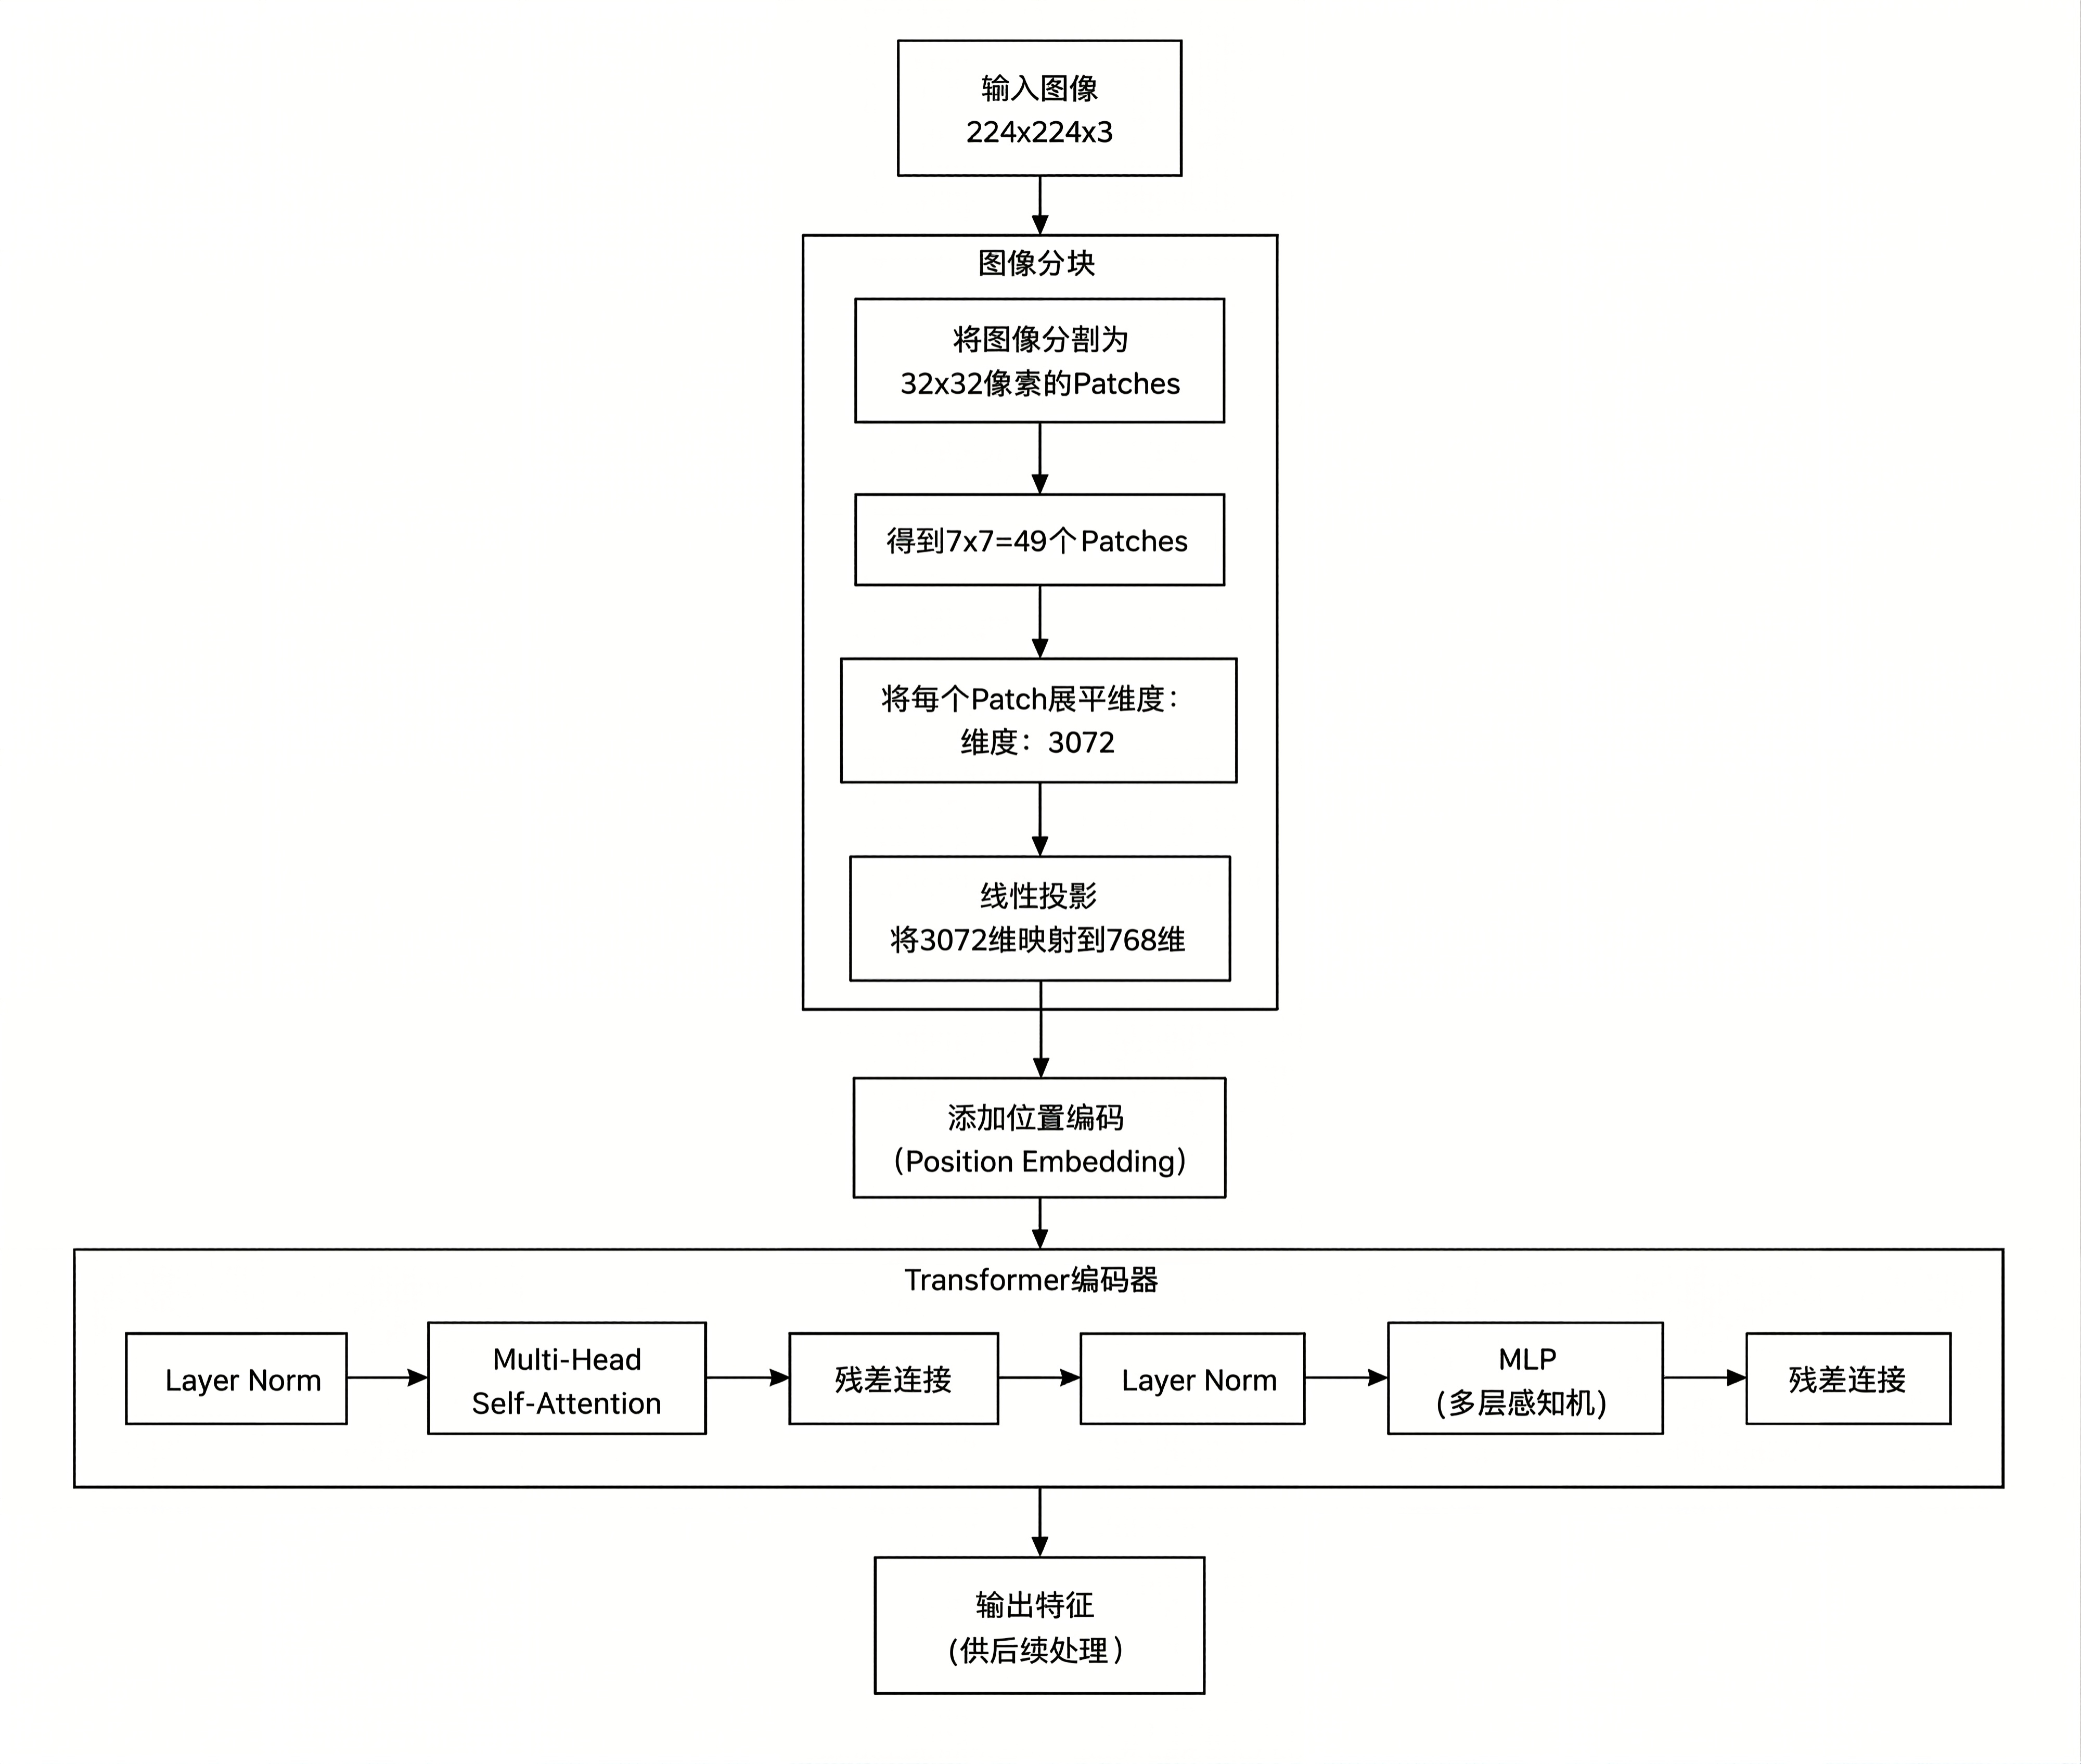
\includegraphics[width=1.05\textwidth]{visionEncoder.jpg}  % 图片与 .tex 文件在同一目录
				\caption{ViT-B/32流程图}
			\end{figure}
			
			可以看出，模型把输入的图像划分成大小固定的一些patch，然后再经过若干层Transformer编码器来做特征建模。ViT有一个特点：每一层都要处理全部的token。所以token数量一旦减少，后面那些层的计算成本就直接跟着降下来了。基于这个观察，裁剪策略的核心问题其实就变成了：在哪一层做裁剪、保留哪些token、删掉哪些token——具体来说，就是在合适的层上，把信息量最大的那些token保留住，冗余的则删掉。
		\subsection{启发式token裁剪实现}
			\subsubsection{基于L2范数的裁剪}
			{\zihao{-4}\setlength{\parindent}{2em}\setlength{\baselineskip}{20pt}\selectfont
				最开始做实验的时候，本文试着用token特征向量的L2范数来当作重要性评分。做法不复杂：每个patch token的特征向量都算一下它的L2范数，计算公式如下：
				\[
				L_2 = \sqrt{x_1^2 + x_2^2 + \cdots + x_n^2}
				\]
				L2范数大的token就认为它包含的信息更多，裁剪的时候优先保留这些。这个方法实现起来简单，算力开销也小，关键是它不需要额外去训练什么东西。\\
				但后面在实际实验里发现，L2范数这种裁剪方式，放到图文检索任务上性能掉得比较明显。尤其是裁剪发生在比较靠前的层时，这个现象更突出。看起来，光靠特征幅值这一个指标，并不足以反映token对任务输出的真实贡献有多大。因为这个原因，后面本文就转用CLS注意力信号来做裁剪依据，效果相对更好一些。
			\subsubsection{基于CLS attention的裁剪}
			{\zihao{-4}\setlength{\parindent}{2em}\setlength{\baselineskip}{20pt}\selectfont
				CLS注意力裁剪的基本想法为：利用CLS token对各个patch token的注意力权重，来衡量每个token的重要性。注意力分数计算公式为：
				\[
				\text{Attention Score} = \frac{QK^T}{\sqrt{d_k}}
				\]
				如果一个patch token跟CLS之间的注意力分数比较高，就说明它对当前全局语义的聚合来说比较关键。反过来，如果注意力很低，那这个区域可能就相对冗余。\\
				具体实现时，在Transformer的某一层里，把CLS token对所有patch token的注意力分数提取出来，然后按分数从高到低排个序。保留排在前面的K个token，剩下的就舍弃掉。K的取值由保留比例决定，计算公式是K = N * r。这里r是保留比例，N是这一层原始的patch token数量。\\
				本文在不同层上对保留比例做了网格搜索，目的是找出一组性能和效率都比较理想的组合。实验结果显示：在图文检索任务上，表现较好的裁剪层是第9层；ScienceQA任务的话，第8层附近效果更好一些；到了Winoground任务，如果在比较早的层就做裁剪，虽然速度会更快，但推理准确率也更容易受到影响。
			\subsubsection{硬裁剪与计算收益}
			{\zihao{-4}\setlength{\parindent}{2em}\setlength{\baselineskip}{20pt}\selectfont
				本文采用的裁剪方式属于硬裁剪。也就是说，被删掉的token在后面的Transformer层里就不再参与任何计算了。这样做的好处是，注意力计算和前馈网络的开销都能实实在在地减下来，从而获得真正的加速效果。如果只是用软掩码而不把token真正移除，那么即便token的权重变小了，计算量其实并没有本质上的下降，也就没法实现真正的推理加速。
		\subsection{gating head的设计与实现}
			\subsubsection{模块结构}
			{\zihao{-4}\setlength{\parindent}{2em}\setlength{\baselineskip}{20pt}\selectfont
				在启发式裁剪的基础上，本文进一步设计了一个轻量级的打分头（gating head），用来学习每个token的重要性分数。打分头结构如下：\\
				\begin{figure}[htbp]
					\centering
					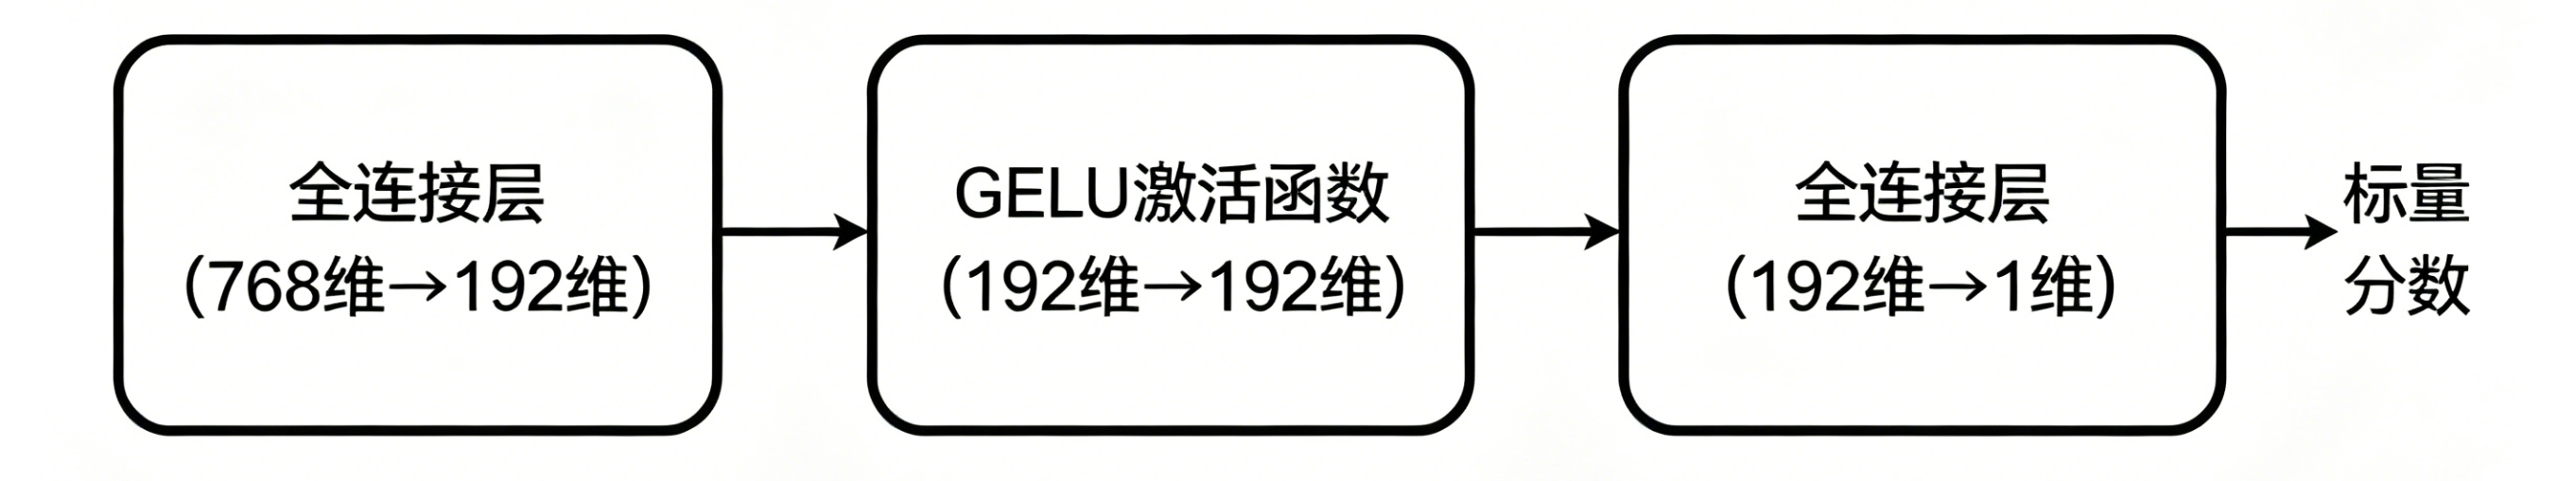
\includegraphics[width=0.7\textwidth]{GatingHead.jpg}  % 图片与 .tex 文件在同一目录
					\caption{GatingHead流程图}
				\end{figure}
				gating head的输入是某一层Transformer输出的patch token特征，输出是每个token对应的一个标量分数。这个分数用来排序，然后决定哪些token被保留。\\
				gating head采用了两层全连接的结构。第一层：把768维的token特征映射到192维；激活函数用的是GELU；第二层：把192维的特征再映射到1维的评分。整体上看，这个结构可以理解为一个寄生在主网络上的轻量评分器。它既能学习token的重要性，又不会让模型的参数量和推理负担增加太多。
			\subsubsection{设计原因}
			把768维压缩到192维，主要考虑了两点。一是减少参数规模，提高训练效率。二是迫使模型提炼出更紧凑的token表示，把更关键的语义信息突出来。中间加入GELU激活函数，是为了引入非线性能力。如果没有非线性，评分模块就只是一个线性映射，表达能力有限，学不好复杂的token重要性判别规则。所以从这个角度看，GELU的引入对于提升gating head的可学习性是必要的。
		\subsection{训练策略设计}
			\subsubsection{软裁剪预训练}
			{\zihao{-4}\setlength{\parindent}{2em}\setlength{\baselineskip}{20pt}\selectfont
			训练阶段，本文没有直接采用硬裁剪，而是先用软裁剪的方式做预训练。所谓软裁剪，就是对token的分数做加权，让低分token的影响变弱，但并不直接把它们删掉。这样做的原因在于：如果训练一开始就直接做硬裁剪，模型很容易因为信息突然缺失而变得不稳定。\\
			软裁剪的好处是，主网络可以逐渐适应token筛选机制，同时gating head也能通过反向传播学到更合理的评分方式。训练的时候，OpenCLIP的文本编码器和视觉骨干的大部分参数都冻结住，只训练gating head。这样评分模块可以专注于学习token的选择策略。
			\subsubsection{硬裁剪推理}
			gating head训练完成之后，在推理阶段就切换到硬裁剪。此时模型不再保留低分token的那些微弱权重，而是直接把没选中的token丢弃掉，只让保留下来的token参与后续Transformer层的计算。这样做可以获得真实的推理加速效果，也能验证训练好的评分机制到底有没有实际应用的价值。
			\subsubsection{微调策略}
			实验中还进一步尝试了对模型做微调。训练阶段模型已经习惯了软裁剪下的微弱信号，但推理阶段硬裁剪会让这些信号直接变成0，所以主网络在推理时可能会出现适应方面的问题。针对这个情况，本文采用的方法是在Flickr30k训练集上做微调，让视觉编码器和gating head共同适应硬裁剪之后的输入分布。\\
			微调过程中，gating head用较小的学习率来更新，保持评分的稳定性。主网络里跟注意力相关的层用相对大一点的学习率，增强它们对裁剪后token集合的适应能力。通过设置不同的训练步数（比如500、1000、1500），比较微调效果对三个任务性能的影响。
		\subsection{多任务实验流程实现}
			\subsubsection{图文检索任务实现}
			{\zihao{-4}\setlength{\parindent}{2em}\setlength{\baselineskip}{20pt}\selectfont
			图文检索任务用的是Flickr30k数据集。每张图像对应五条人工标注的文本描述。实验时在测试集的1000张图像上直接评测模型性能，统计Recall@1、Recall@5和Recall@10这几个指标。先测原始OpenCLIP模型作为baseline，再在不同裁剪层和不同保留比例下做对比实验，最后确定比较优的裁剪配置。
			\subsubsection{视觉问答任务实现}
			视觉问答任务用的是ScienceQA数据集。ScienceQA里每个样本包含一个问题、若干个选项，以及正确答案的索引。本文只拿那些包含图像的样本来做测试。先在验证集的小样本上做网格搜索，快速筛选出较好的裁剪层和保留比例；然后到全量验证集和测试集上做评测，统计准确率和推理时间，分析裁剪对答题效果的影响。
			\subsubsection{图文推理任务实现}
			图文推理任务用的是Winoground数据集。这个数据集的样本量不大，但难度比较高，尤其考验模型对图像和文本之间细粒度对应关系的判断能力。本文在全量样本上做测试，在不同层和不同保留比例下分析裁剪对推理准确率和速度的影响。
		\subsection{评价指标设计}
			{\zihao{-4}\setlength{\parindent}{2em}\setlength{\baselineskip}{20pt}\selectfont
			本文主要从性能和效率两个维度来评价裁剪方法。
			\subsubsection{性能指标}
			图文检索这边用Recall@1、Recall@5、Recall@10。视觉问答用分类准确率。图文推理用匹配准确率，或者说任务里规定的综合准确率指标。
			\subsubsection{效率指标}
			平均推理时间、每秒处理的样本数（samples/sec）、加速比（相对于baseline的时间下降比例），还有token保留比例与后续层计算量的下降幅度。
		\subsection{实现中的若干技术细节}
			\subsubsection{文本特征缓存}
			{\zihao{-4}\setlength{\parindent}{2em}\setlength{\baselineskip}{20pt}\selectfont
			为了提高实验效率，本文在多任务评测中对文本特征做了缓存复用。因为文本编码器在不同的裁剪配置下通常是不变的，所以可以把文本特征一次性计算好放在内存里反复使用，这样能减少重复推理的开销。
			\subsubsection{单进程推理}
			实验采用单进程的方式执行。这样做的目的是避免多进程切换和频繁加载模型权重带来的额外开销。模型只加载一次，然后在内存里完成多个配置的评测，有助于提升网格搜索的整体效率。
			\subsubsection{keep ratio与裁剪层选择}
			实验结果显示，不同任务对裁剪层和保留比例的敏感性是不一样的。因此本文在实现中保留了可配置的接口，可以灵活指定裁剪发生在哪一层、保留比例是多少，以及是否启用硬裁剪或软裁剪。
	\section{研究结果与分析}	
	{\zihao{-4}\setlength{\parindent}{2em}\setlength{\baselineskip}{20pt}\selectfont
		本文以OpenCLIP（ViT-B/32）作为视觉编码器，提出了一种基于CLS注意力分数的自适应Token裁剪方法。该方法在图文检索、视觉问答、图文推理这三个多模态理解任务上做了系统性实验，目的是验证它在性能与效率之间的平衡能力，以及跨任务的泛化效果。此外，还进一步引入了一个可训练的Gating Head来优化裁剪策略，最终形成了一套完整的自适应Token裁剪方案。下面从四个维度对实验结果展开论述：单任务上的实验结果、跨任务的Pareto最优分析、可学习裁剪模块的实际效果，以及一些关键现象的观察分析。
		\subsection{基于CLS注意力的启发式Token裁剪单任务结果}
			\subsubsection{图文检索任务(Flickr30k)}
			在Flickr30k测试集1000张图像上，无裁剪基线模型的检索指标为R@1=0.845、R@5=0.960、R@10=0.985，单张图像编码耗时7.2ms。实验首先对比Token重要性评估方式：采用L2范数进行裁剪时各层性能下降明显，在第9层保留50\% Token时R@1仅为0.781；因为L2范数大只能说明图像比较活跃，未必是关键区域，也有可能是噪声区域，因此弃用L2范数作为打分依据。\\
			后续改用以CLS对Patch Token的注意力权重作为重要性依据，这样能够更稳定地保留关键语义信息。扫描在keep ratio=0.5时各个剪枝层的效果，结果如下：
			\par
			\setlength{\tabcolsep}{12pt}      % 列间距
			\renewcommand{\arraystretch}{1.3}  % 行高
			\begin{longtable}{|c|c|c|c|}
				\caption{keep ratio=0.5时各个裁剪层的效果}  % 添加标题
				\label{tab:fixKeepRatio} \\

				\hline
				剪枝层 & R@1 & R@5 & R@10 \\
				\hline
				\endfirsthead
				
				\caption{keep ratio=0.5时各个裁剪层的效果(续)} \\
				\hline
				剪枝层 & R@1 & R@5 & R@10 \\
				\hline
				\endhead
				
				\hline
				\endfoot
				
				Baseline & 0.845 & 0.960 & 0.985 \\
				\hline
				layer4 & 0.756 & 0.921 & 0.954 \\
				\hline
				layer5 & 0.746 & 0.914 & 0.950 \\
				\hline
				layer6 & 0.773 & 0.934 & 0.971 \\
				\hline
				layer7 & 0.815 & 0.935 & 0.974 \\
				\hline
				layer8 & 0.814 & 0.954 & 0.981 \\
				\hline
				layer9 & 0.833 & 0.957 & 0.980 \\
				\hline
				layer10 & 0.822 & 0.953 & 0.982 \\
				\hline				
				
			\end{longtable}
			\par
			接着再在layer9上扫描各个keep ratio的效果：
			\par
			\setlength{\tabcolsep}{12pt}      % 列间距
			\renewcommand{\arraystretch}{1.3}  % 行高
			\begin{longtable}{|c|c|c|c|}
				\caption{Layer=9时各个保留比例的效果}  % 添加标题
				\label{tab:fixLayer} \\
				
				\hline
				keepRatio & R@1 & R@5 & R@10 \\
				\hline
				\endfirsthead
				
				\caption{Layer=9时各个保留比例的效果(续)} \\
				\hline
				keepRatio & R@1 & R@5 & R@10 \\
				\hline
				\endhead
				
				\hline
				\endfoot
				
				Baseline & 0.845 & 0.960 & 0.985 \\
				\hline
				0.90 & 0.848 & 0.962 & 0.984 \\
				\hline
				0.75 & 0.844 & 0.962 & 0.984 \\
				\hline
				0.60 & 0.834 & 0.960 & 0.983 \\
				\hline
				0.50 & 0.833 & 0.957 & 0.980 \\
				\hline
				0.25 & 0.725 & 0.903 & 0.951 \\
				\hline				
				
			\end{longtable}
			\par
			根据上述网格搜索结果，可以得到在不显著降低准确率的前提下加速比最高的组合为第9层、保留比例0.5。此时模型R@1=0.833、R@5=0.957、R@10=0.980，与基线相比仅分别下降0.012、0.003、0.005；同时后续层Token数量减半，视觉编码计算量降低约50\%，实现显著推理加速。结果表明，CLS注意力能够有效刻画图像Token的重要程度，在ViT中后层实施中等比例裁剪，可在图文检索任务上实现性能与效率的良好平衡。
			\subsubsection{视觉问答任务(ScienceQA)}
			在ScienceQA带图像验证集（2097条）与测试集（2017条）上，直接沿用CLS注意力裁剪策略，未进行任务特定微调。由于全量搜索耗时太久，首先通过在小样本验证集max=500时，进行网格搜索：
			\par
			\setlength{\tabcolsep}{12pt}      % 列间距
			\renewcommand{\arraystretch}{1.3}  % 行高
			\begin{longtable}{|c|c|c|c|}
				\caption{小样本时的网格搜索}  % 添加标题
				\label{tab:max=500} \\
				
				\hline
				裁剪层 & keepRatio & acc & speedup \\
				\hline
				\endfirsthead
				
				\caption{小样本时的网格搜索(续)} \\
				\hline
				裁剪层 & keepRatio & acc & speedup \\
				\hline
				\endhead
				
				\hline
				\endfoot
				
				Baseline & 无 & 0.3600 & 1.000 \\
				\hline
				7 & 0.3 & 0.3950 & 2.523 \\
				\hline
				7 & 0.5 & 0.3750 & 3.533 \\
				\hline
				7 & 0.7 & 0.3600 & 3.447 \\
				\hline
				8 & 0.3 & 0.4050 & 3.764 \\
				\hline
				8 & 0.5 & 0.3800 & 4.125 \\
				\hline
				8 & 0.7 & 0.3700 & 4.808 \\
				\hline
				9 & 0.3 & 0.4000 & 4.710 \\
				\hline
				9 & 0.5 & 0.3500 & 4.751 \\
				\hline
				9 & 0.7 & 0.3550 & 5.001 \\
				\hline
				10 & 0.3 & 0.3900 & 3.115 \\
				\hline
				10 & 0.5 & 0.3800 & 3.253 \\
				\hline
				10 & 0.7 & 0.3650 & 3.599 \\
				\hline
				11 & 0.3 & 0.3600 & 4.045 \\
				\hline
				11 & 0.5 & 0.3600 & 3.711 \\
				\hline
				11 & 0.7 & 0.3600 & 4.619 \\
				\hline				
				
			\end{longtable}
			\par
			小样本网格搜索结果显示，准确率最优组合为第8层、保留比例0.3，加速比最优组合为第9层、保留比例0.7。\\
			接着再在上述两个配置上跑全量验证集：\\
			\setlength{\tabcolsep}{12pt}      % 列间距
			\renewcommand{\arraystretch}{1.3}  % 行高
			\begin{longtable}{|c|c|c|c|}
				\caption{特定配置下全量验证集}  % 添加标题
				\label{tab:fullVal} \\
				
				\hline
				裁剪层 & keepRatio & acc & speedup \\
				\hline
				\endfirsthead
				
				\caption{特定配置下全量验证集(续)} \\
				\hline
				裁剪层 & keepRatio & acc & speedup \\
				\hline
				\endhead
				
				\hline
				\endfoot
				
				Baseline & 无 & 0.3887 & 1.000 \\
				\hline
				8 & 0.3 & 0.3896 & 1.307 \\
				\hline
				9 & 0.7 & 0.3887 & 1.533 \\
				\hline				
				
			\end{longtable}
			全量验证集测试表明：采用第8层、保留比例0.3时，验证集准确率由0.3887提升至0.3896，加速比1.31×；采用第9层、保留比例0.7时，验证集与测试集准确率均保持0.3887不变，加速比达到1.53×。\\
			接着我又在全量测试集上验证上述情况：\\
			\setlength{\tabcolsep}{12pt}      % 列间距
			\renewcommand{\arraystretch}{1.3}  % 行高
			\begin{longtable}{|c|c|c|c|}
				\caption{特定配置下全量测试集}  % 添加标题
				\label{tab:fullTest} \\
				
				\hline
				裁剪层 & keepRatio & acc & speedup \\
				\hline
				\endfirsthead
				
				\caption{特定配置下全量测试集(续)} \\
				\hline
				裁剪层 & keepRatio & acc & speedup \\
				\hline
				\endhead
				
				\hline
				\endfoot
				
				Baseline & 无 & 0.4170 & 1.000 \\
				\hline
				8 & 0.3 & 0.4254 & 1.153 \\
				\hline
				9 & 0.7 & 0.4189 & 1.177 \\
				\hline				
				
			\end{longtable}
			测试集与验证集上的结论一致，CLS注意力裁剪可在几乎不损失精度甚至小幅提升精度的前提下，为视觉问答任务提供稳定推理加速，这与ScienceQA对图像细粒度细节依赖度较低的特点密切相关。
			\subsubsection{图文推理任务(Winoground)}
			Winoground包含400条细粒度空间关系推理样本，对局部视觉结构高度敏感。对裁剪层和保留比例进行网格搜索，结果如下：\\
			
			\setlength{\tabcolsep}{12pt}      % 列间距
			\renewcommand{\arraystretch}{1.1}  % 行高
			
			\begin{longtable}{|c|c|c|c|}
				\caption{全量网格搜索}  % 添加标题
				\label{tab:fullData} \\
				\hline
				裁剪层 & keepRatio & acc & speedup \\
				\hline
				\endfirsthead
				
				%续表头
				\caption{全量网格搜索(续)} \\
				\hline
				裁剪层 & keepRatio & acc & speedup \\
				\hline
				\endhead
				
				\hline
				\endfoot
				
				%表格内容
				Baseline & 无 & 0.3100 & 1.000 \\
				\hline
				6 & 0.1 & 0.2200 & 1.403 \\
				\hline
				6 & 0.3 & 0.2700 & 1.677 \\
				\hline
				6 & 0.5 & 0.3075 & 1.650 \\
				\hline
				6 & 0.7 & 0.2975 & 1.926 \\
				\hline
				6 & 0.9 & 0.3050 & 2.188 \\
				\hline
				7 & 0.1 & 0.2200 & 1.796 \\
				\hline
				7 & 0.3 & 0.2550 & 1.838 \\
				\hline
				7 & 0.5 & 0.2900 & 1.761 \\
				\hline
				7 & 0.7 & 0.2950 & 1.850 \\
				\hline
				7 & 0.9 & 0.3100 & 1.684 \\
				\hline
				8 & 0.1 & 0.2225 & 1.918 \\
				\hline
				8 & 0.3 & 0.2750 & 1.792 \\
				\hline
				8 & 0.5 & 0.2975 & 1.711 \\
				\hline
				8 & 0.7 & 0.3000 & 1.629 \\
				\hline
				8 & 0.9 & 0.3150 & 1.989 \\
				\hline
				9 & 0.1 & 0.2600 & 1.850 \\
				\hline
				9 & 0.3 & 0.2850 & 1.638 \\
				\hline
				9 & 0.5 & 0.2950 & 1.637 \\
				\hline
				9 & 0.7 & 0.3050 & 1.685 \\
				\hline
				9 & 0.9 & 0.3150 & 1.982 \\
				\hline
				10 & 0.1 & 0.2250 & 1.938 \\
				\hline
				10 & 0.3 & 0.2800 & 1.713 \\
				\hline
				10 & 0.5 & 0.3050 & 1.763 \\
				\hline
				10 & 0.7 & 0.3025 & 1.786 \\
				\hline
				10 & 0.9 & 0.3125 & 1.751 \\
				\hline
				11 & 0.1 & 0.3100 & 1.879 \\
				\hline
				11 & 0.3 & 0.3100 & 1.807 \\
				\hline
				11 & 0.5 & 0.3100 & 1.870 \\
				\hline
				11 & 0.7 & 0.3100 & 1.800 \\
				\hline
				11 & 0.9 & 0.3100 & 1.873 \\
				\hline
			\end{longtable}
		
			全量网格搜索结果显示，激进裁剪会显著降低准确率，而保守裁剪可在保持性能的同时实现加速。其中第8层、保留比例0.9的配置表现最优，准确率由0.310提升至0.315，加速比1.99×；第6层、保留比例0.9的配置加速比最高，达到2.19×，准确率仅降至0.305。\\
			实验中观察到保留比例0.9的耗时低于0.7的反常现象，主要原因包括裁剪带来的额外注意力计算开销、GPU Tensor Core对2的幂次Token数的对齐优化，以及小样本计时带来的波动。多次计时平均后，上述结论依然稳定。结果表明，图文推理任务对Token裁剪更为敏感，仅适合在浅层实施保守裁剪。
		\subsection{跨任务Pareto最优配置分析}
			为获得适用于图文检索、视觉问答与图文推理的通用裁剪方案，以检索召回率、任务准确率及平均推理时间为优化目标，对8组候选配置进行Pareto最优筛选，最终得到3组非支配解：Layer6+ratio0.9、Layer8+ratio0.9、Layer9+ratio0.9，数据如下表：\\
			\setlength{\tabcolsep}{3pt}      % 列间距
			\renewcommand{\arraystretch}{1.1}  % 行高
			\begin{longtable}{|c|c|c|c|c|c|c|c|c|}
				\caption{三组非支配解}  % 添加标题
				\label{tab:pareto} \\
				
				\hline
				裁剪层 & keepRatio & 图文检索(平均) & 图文问答 & 图文推理 & cost & R@1 & R@5 & R@10 \\
				\hline
				\endfirsthead
				
				\caption{三组非支配解(续)} \\
				\hline
				裁剪层 & keepRatio & 图文检索(平均) & 图文问答 & 图文推理 & cost & R@1 & R@5 & R@10 \\
				\hline
				\endhead
				
				\hline
				\endfoot
				
				6 & 0.9 & 0.9167 & 0.4125 & 0.3050 & 0.3094 & 0.8200 & 0.9540 & 0.9760 \\
				\hline
				9 & 0.9 & 0.9180 & 0.3750 & 0.3150 & 0.3811 & 0.8260 & 0.9500 & 0.9780 \\
				\hline
				8 & 0.9 & 0.9180 & 0.3800 & 0.3150 & 0.4403 & 0.8250 & 0.9510 & 0.9780 \\
				\hline				
				
			\end{longtable}
			综合性能与效率权衡，本文选取 Layer6+ratio0.9作为跨任务基准配置。
			该配置在三项任务中均保持可接受的性能损失，同时实现稳定加速：图文检索R@1为 0.820，ScienceQA 测试集准确率0.4125，Winoground准确率0.305。Pareto分析表明，自适应Token裁剪不存在适用于所有场景的固定参数，需根据任务特性动态调整：检索任务适合在中后层进行中等比例裁剪，问答任务可在多层级灵活裁剪，推理任务则更适合浅层保守裁剪。
		\subsection{可学习Gating Head裁剪模块结果}
			为进一步提升Token重要性评估精度，本文在跨任务基准Layer6+ratio0.9的基础上，引入轻量级可训练Gating Head替代启发式CLS注意力打分。Gating Head由两层全连接与GELU激活构成，将768维Token特征映射为一维重要性分数，训练阶段采用软裁剪保证可导性，推理阶段切换为硬裁剪以降低计算量。\\
			仅训练Gating Head并直接采用硬裁剪推理时，图文检索性能与启发式方法接近，图文推理准确率由0.305提升至0.3175，但ScienceQA测试集准确率由0.4125降至0.3550，出现明显性能下降。其主要原因是训练阶段的软裁剪与推理阶段的硬裁剪存在分布差异，主干网络未适应真实Token丢弃。\\
			为缓解上述域偏移问题，本文采用分层微调策略：冻结文本编码器与视觉编码器前6层，微调视觉编码器后5层、投影层及Logit Scale，并以小学习率更新或固定Gating Head。分别以500、1000、1500步进行微调，视觉问答精度显著回升，图文推理保持高性能，图文检索指标稳定，三项任务均维持1.5倍以上的推理加速。最终的结果汇总如下表：\\
			\setlength{\tabcolsep}{6pt}      % 列间距
			\renewcommand{\arraystretch}{1.3}  % 行高
			\begin{longtable}{|c|c|c|c|c|c|}
				\caption{使用打分头之后的效果对比}  % 添加标题
				\label{tab:gating head} \\
				
				\hline
				设置 & R@1 & R@5 & R@10 & 图文问答 & 图文推理 \\
				\hline
				\endfirsthead
				
				\caption{使用打分头之后的效果对比(续)} \\
				\hline
				设置 & R@1 & R@5 & R@10 & 图文问答 & 图文推理 \\
				\hline
				\endhead
				
				\hline
				\endfoot
				
				直接启发式裁剪 & 0.8200 & 0.9540 & 0.9760 & 0.4050 & 0.3050 \\
				\hline
				训练打分头+硬裁剪 & 0.8200 & 0.9530 & 0.9770 & 0.3550 & 0.3175 \\
				\hline
				微调500steps & 0.8850 & 0.9810 & 0.9930 & 0.4100 & 0.3150 \\
				\hline
				微调1000steps & 0.8990 & 0.9870 & 0.9980 & 0.4000 & 0.3075 \\
				\hline
				微调1500steps & 0.8960 & 0.9860 & 0.9960 & 0.3900 & 0.3075 \\
				\hline				
				
			\end{longtable}
			可以得出可学习Gating Head裁剪在跨任务场景下全面优于启发式方法，有效提升了细粒度推理任务的适配能力。
		\subsection{关键结果分析与讨论}
			\subsubsection{CLS注意力的有效性}
				CLS注意力是模型自监督训练过程中自然生成的重要性信号，无需额外标注、训练或模型修改，即可作为通用Token裁剪依据。在三项多模态任务上的实验一致证明，该方式能够稳定识别关键视觉Token，为零样本ViT推理加速提供轻量解决方案。
			\subsubsection{任务敏感性差异}
				图文检索依赖全局语义对齐，对细节不敏感，支持在中后层裁剪50\% Token，计算量下降显著；视觉问答的图像信息冗余度高，裁剪后可实现无损甚至增益加速；图文推理依赖空间关系与局部结构，对Token丢失最为敏感，仅支持浅层、高保留比例的保守裁剪。任务敏感性差异表明，自适应Token裁剪应根据任务对视觉细节的依赖程度动态选择裁剪位置与保留比例。
			\subsubsection{软-硬裁剪的训练与推理适配}
				软裁剪确保训练过程可导且稳定，硬裁剪实现真实计算量下降。结合主干网络分层微调，可有效缩小训练与推理之间的分布差异，使可学习裁剪模块在部署阶段稳定发挥性能，为ViT动态结构的落地提供可行路径。
			\subsubsection{效率优化价值}
				通过单进程缓存文本特征、复用模型权重，多配置网格搜索的整体效率提升约1.25倍。结合Token裁剪带来的计算量下降，形成算法层面与工程层面的双重加速，更适合端侧与低资源环境部署。
		\subsection{本节小结}
			基于CLS注意力的ViT自适应Token裁剪，可在无额外训练与标注的条件下，在图文检索、视觉问答、图文推理任务上实现性能无损或微损下的有效加速，加速比介于1.3×至2.19×之间。跨任务Pareto最优配置验证了策略的任务适配性，为多场景部署提供参数选择依据。引入可学习Gating Head并配合分层微调，可进一步提升模型在细粒度推理任务上的表现，实现跨任务均衡优化。实验结果表明，自适应Token裁剪并非固定参数的静态裁剪，而是应结合任务特性与结构位置动态实施的动态优化机制。
	\section{结论}
	{\zihao{-4}\setlength{\parindent}{2em}\setlength{\baselineskip}{20pt}\selectfont
		针对多模态理解任务中Vision Transformer存在计算量大、推理效率偏低的问题，本文围绕ViT自适应Token裁剪方法展开研究。以OpenCLIP(ViT-B/32)为基础模型，提出一种基于CLS注意力分数的无训练Token重要性评估手段，并进一步设计轻量级可学习Gating Head以优化裁剪策略。在图文检索、视觉问答、图文推理三项任务上完成系统性实验验证。结果表明，所提自适应裁剪方案可在模型性能基本不损失的前提下实现视觉编码器计算量显著下降，并具备良好跨任务泛化能力与工程实用价值。\\
	{\zihao{-4}\setlength{\parindent}{0em}\setlength{\baselineskip}{20pt}\selectfont
		本文主要研究结论可归纳为以下几点：\\
		1)CLS注意力可作为通用无监督Token重要性指标。CLS对于Patch Token的注意力权重来源于模型自监督学习中天然形成的语义重要性信号，无需额外标注、数据或训练开销即可有效定位关键视觉区域。在三项多模态任务中，该方案均明显优于传统L2范数打分策略，表现出稳定通用的Token筛选能力。\\
		2)自适应Token裁剪能够在模型性能与推理效率之间实现有效平衡。图文检索任务中，第9层保留50\%Token可使计算量降低约50\%，召回率仅轻微下降；ScienceQA视觉问答任务可实现1.53倍加速且准确率无损，部分配置甚至出现小幅提升；Winoground图文推理任务采用浅层高比例保守裁剪可获得近2倍加速，且准确率不降反升。以上结果充分验证了动态裁剪策略的有效性。\\
		3)不同任务对Token裁剪的敏感程度差异明显。图文检索依赖全局语义匹配，适合在中后层进行中等比例裁剪；视觉问答图像具有较高信息冗余度，可支持相对激进的裁剪策略；图文推理依赖空间关系与细粒度结构信息，对Token丢失最为敏感，仅适合在浅层实施高保留比例的保守裁剪。这一规律可为多模态模型部署提供参数选取依据。\\
		4)可学习Gating Head配合分层微调有利于提升跨任务泛化性能。本文设计的轻量级Gating Head可通过数据驱动方式学习Token重要性，将软裁剪用于训练、硬裁剪用于推理，并采用分层微调缓解训练与推理之间的分布差异，使可学习裁剪在细粒度推理任务中表现更优，同时在检索与问答任务中保持稳定，实现跨任务均衡优化。\\
		5)工程优化有效提升了方法的落地可行性。通过模型权重复用、文本特征缓存等流程层面的优化，多配置网格搜索效率提升1.25倍。结合Token裁剪带来的计算量下降，所提方法在边缘设备及低算力平台场景中具备良好应用前景。
		\subsection{主要创新点}
		{\zihao{-4}\setlength{\parindent}{0em}\setlength{\baselineskip}{20pt}\selectfont
			1)提出基于CLS注意力的零样本ViT Token裁剪方法，无需训练与标注即可完成自适应Token重要性评估，具备轻量化与易部署特点。\\
			2)在图文检索、视觉问答、图文推理三项特性差异显著的多模态任务上开展全面验证，揭示了任务敏感性与裁剪位置、保留比例之间的对应规律。\\
			3)构建了包含Gating Head可学习打分、软硬裁剪结合、分层微调的完整流程，解决了训练与推理分布偏移问题，提升了跨任务鲁棒性。\\
			4)基于Pareto最优给出了跨任务通用裁剪配置，为实际系统提供了可直接采用的性能–效率折中方案。
		\subsection{未来工作展望}
		{\zihao{-4}\setlength{\parindent}{0em}\setlength{\baselineskip}{20pt}\selectfont
			1)探索多层CLS注意力融合打分方式，以提升细粒度及复杂场景下的裁剪稳定性。\\
			2)将自适应Token裁剪与量化、知识蒸馏等技术相结合，构建多级模型压缩框架。\\
			3)扩展至更大规模ViT模型以及视频理解、跨模态生成等任务，进一步验证方法的通用性。\\
			4)研究基于图像内容的动态Token保留策略，实现计算资源分配与输入复杂程度的自适应匹配。\\
			5)开展端侧及嵌入式平台部署实验，验证真实场景中推理速度、内存占用及功耗收益。
	\renewcommand{\refname}{} %隐藏默认生成的“参考文献”
	\section{参考文献}
	\vspace{-4em} %往上移动位置 方便观看
	\begin{thebibliography}{99}
		\markboth{第八章\ 参考文献}{第八章\ 参考文献}
		
		\bibitem{radford2021} Radford A, Kim J W, Hallacy C, et al. Learning transferable visual models from natural language supervision [C] // International Conference on Machine Learning. PMLR, 2021: 8748-8763.
		
		\bibitem{cherti2022} Cherti M, Beaumont R, Wightman R, et al. Reproducible scaling laws for contrastive language-image learning [J]. arXiv preprint arXiv:2212.07143, 2022.
		
		\bibitem{liu2023} Liu X C, Wu T Y, Guo G D. Adaptive sparse vit: Towards learnable adaptive token pruning by fully exploiting self-attention [C] // Proceedings of the Thirty-Second International Joint Conference on Artificial Intelligence. 2023.
		
		\bibitem{yu2024} Yu H, Wang W, Li Y, et al. ViTCoP: Accelerating Large Vision-Language Models via Visual and Textual Semantic Collaborative Pruning [C] // Proceedings of the AAAI Conference on Artificial Intelligence. 2024.
		
		\bibitem{chen2026} Chen J, Gong K, Yu T, et al. Rényi Entropy: A New Token Pruning Metric for Vision Transformers [J]. arXiv preprint arXiv:2603.27900, 2026.
		
		\bibitem{dosovitskiy2020} Dosovitskiy A, Beyer L, Kolesnikov A, et al. An image is worth 16x16 words: Transformers for image recognition at scale [J]. arXiv preprint arXiv:2010.11929, 2020.
		
		\bibitem{zhang2025} 张宇, 彭书俊, 林新涵, 等. ViT-CAAC：面向视觉Transformer的贡献感知自适应压缩框架 [J]. 计算机研究与发展, 2025.
		
		\bibitem{young2014} Young P, Lai A, Hodosh M, et al. From image descriptions to visual denotations: New similarity metrics for semantic inference over event descriptions [J]. Transactions of the Association for Computational Linguistics, 2014, 2: 67-78.
		
	\end{thebibliography}
	
	\section{致谢}
	{\zihao{-4}\setlength{\parindent}{2em}\setlength{\baselineskip}{20pt}\selectfont
		时光飞逝，每次刷卡进校，看到闸机上显示“有效期至2026”，总觉得那个年份还很遥远。如今距离毕业已不到两个月，我在复旦的本科生涯也即将画上句号。回首从2019年入学，2020年入伍，2022年退伍返校，再到2026年终于要本科毕业，心里感慨良多。\\
		首先，衷心感谢陈智能老师对我的指导。从选题的反复推敲，到实验方向的把握，陈老师都给了我很多实实在在的帮助。尤其是我在实验卡住的时候，陈老师总能一针见血地指出问题所在。他教给我的不光是知识，更是做学问的态度和作为一名复旦人应有的担当。\\
		同时，也感谢复旦大学计算与智能创新学院的各位授课老师，是你们的教导为我后续的科研打下了扎实的基础。感谢我的室友杨智雄和贾伦，谢谢你们在学习上给我的帮助，也谢谢你们在我备考期间生活上的包容。这些点点滴滴，都会是我青春里最珍贵的记忆。感谢我的家人，一直在我身后默默支持、无条件地信任我，你们永远是我最坚实的后盾。\\
		最后，感谢那个始终没有放弃的自己。
		
	% ========================
	% 3. 最后一页：结尾页（cover.pdf 第2页）
	% ========================
	
\includepdf[pages=2]{cover.pdf}
	
\end{document}